\section{Auswertung}

\subsection{Bestimmung der Schallgeschwindigkeit mit dem Impuls-Echo-Verfahren}
Die aufgenommenen zeitlichen Abstände der beobachteten Spannungsimpulse sind in Tabelle \ref{tab: c_echo}
augetragen. Gemäß
\begin{equation}
  \frac{\Delta t}{2} = \frac{1}{2}\left(t_2 - t_1\right)
\end{equation}
berechnen sich die halben zeitlichen Differenzen der Impulse. Die Daten werden verwendet um eine
lineare Regression an die Funktion der Form
\begin{equation}
  s \left(\frac{\Delta t}{2}\right) = c\ua{E} \frac{\Delta t}{2} + b\ua{E}
\end{equation}
durchzuführen. Für die Schallgeschwindigkeit in Acryl $c\ua{E}$ und den Abszissenabschnitt $b\ua{E}$
ergeben sich
\begin{align}
  \begin{aligned}
    c\ua{E} &= \SI{+2.79(2)e+03}{\meter\per\second} \\
    b\ua{E} &= \SI{-1.6(5)}{\milli\meter}.
    \label{eq: params_echo}
  \end{aligned}
\end{align}
\begin{table}[H] 
\centering 
\caption{Daten zur Bestimmung der Schallgeschwindigkeit in Acryl mit der Impuls-Echo-Methode. Laufstrecke $s$, Zeitlicher Abstand der Pulse zum Ursprung $t_1$, $t_2$ und berechnete halbe Zeitdifferenz $\frac{\Delta t }{2}$.} 
\label{tab: c_echo} 
\begin{tabular}{S S S S } 
\toprule  
{$s / \si{\milli\meter}$} & {$t_1 / \si{\micro\second}$} &  {$t_2 / \si{\micro\second}$}& {$\frac{\Delta t }{2} / \si{\micro\second}$}  \\ 
\midrule  
 31.10  & 0.4  & 23.9  & 11.8\\ 
40.00  & 0.3  & 29.8  & 14.8\\ 
61.68  & 0.4  & 46.3  & 22.9\\ 
72.00  & 1.1  & 53.4  & 26.1\\ 
80.60  & 1.1  & 59.8  & 29.3\\ 
111.78  & 1.3  & 82.6  & 40.6\\ 
120.80  & 1.3  & 88.9  & 43.8\\ 
\bottomrule 
\end{tabular} 
\end{table}
\begin{figure}[H]
  \centering
  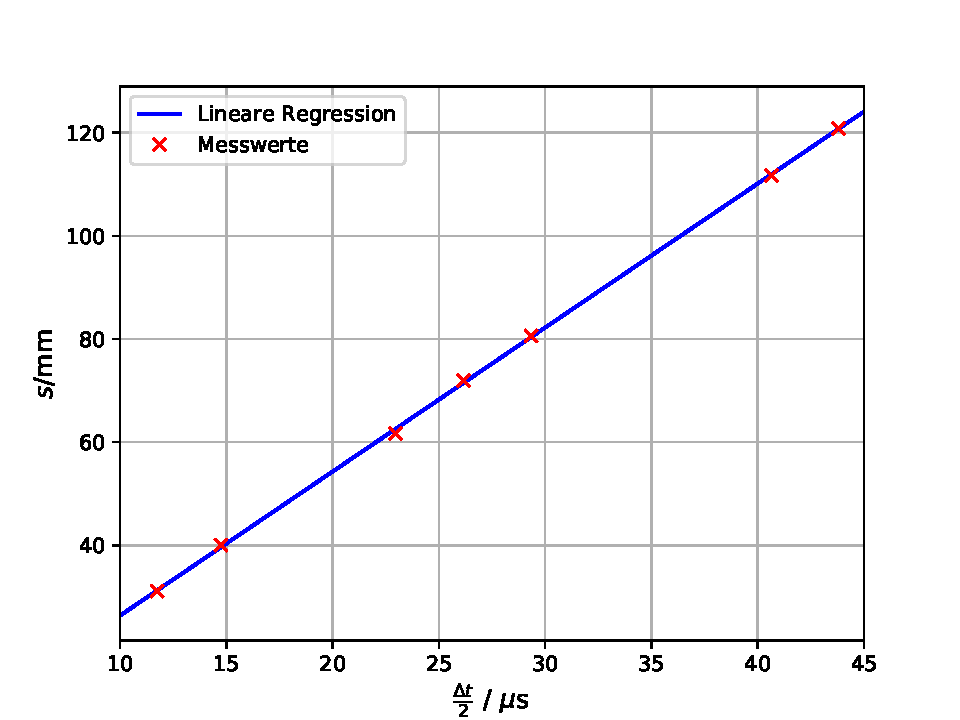
\includegraphics[width = 0.7\textwidth]{../Messdaten/plots/schallgeschwindigkeit.pdf}
  \caption{Graphische Darstellung der Messwertpaare zur Bestimmung der Schallgeschwindigkeit
  mit der Impuls-Echo-Methode (Strecke $s$ und Laufzeit $\frac{\Delta t}{2}$) sowie der linearen Regression.}
  \label{fig: c_echo}
\end{figure}


\subsection{Bestimmung der Schallgeschwindigkeit mit dem Durchschallungsverfahren}
Die aufgenommenen Laufzeiten $t$ des Ultraschalls für die verwendeten Acrylzylinder der Länge $s$ sind
in Tabelle \ref{tab: c_durchsschallung} aufgetragen. Eine Auftragung der Distanzen gegen die Laufzeit sowie
der linearen Regression ist in Abbildung \ref{fig: c_durchschallung} einzusehen. Für die Geschwindigkeit $c\ua{D}$ %ref
als Steigung der bestimmten Regressiongerade bzw. den Abszissenabschnitt $b\ua{D}$ ergeben sich
\begin{align}
  \begin{aligned}
    c\ua{D} &= \SI{+2.74(3)e+03}{\meter\per\second}\\
    b\ua{D} &= \SI{-3.7(9)}{\milli\meter}.
  \end{aligned}
\end{align}
Mit den Ergebnissen des Impuls-Echo Verfahrens ergeben sich die Mittelwerte $c\ua{mid}$ und $b\ua{mid}$ zu
\begin{align}
  \begin{aligned}
  c\ua{mid} &= \SI{+2.76(2)e+03}{\meter\per\second}. \\
  b\ua{mid} &= \SI{-2.6(5)}{\milli\meter}.
\end{aligned}
\end{align}
Der Literatur \cite{olympus} wird folgender Wert entnommen
\begin{equation}
  c\ua{lit} = \SI{2.73e3}{\meter\per\second}.
  \label{eq: c_lit}
\end{equation}

\begin{table} 
\centering 
\caption{Daten zur Bestimmung der Schallgeschwindigkeit in Acryl mit der Durchschallungsmethode. Laufstrecke $s$ und Laufzeit $t$.} 
\label{tab: c_durchsschallung} 
\begin{tabular}{S S } 
\toprule  
{$s / \si{\milli\meter}$} & {$t / \si{\micro\second}$}  \\ 
\midrule  
 31.10  & 12.9\\ 
40.00  & 15.8\\ 
61.68  & 23.9\\ 
80.60  & 30.5\\ 
102.36  & 39.2\\ 
120.80  & 45.3\\ 
\bottomrule 
\end{tabular} 
\end{table}
\begin{figure}[H]
  \centering
  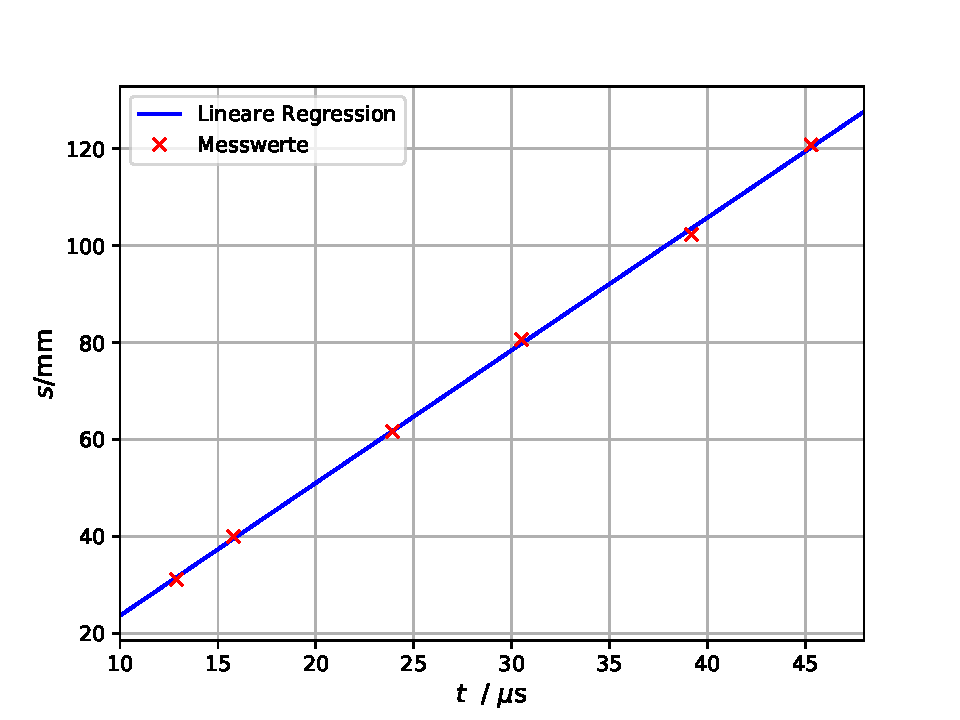
\includegraphics[width = 0.7\textwidth]{../Messdaten/plots/schallgeschwindigkeit_durchschallung.pdf}
  \caption{Graphische Darstellung der Messwertpaare zur Bestimmung der Schallgeschwindigkeit
  mit der Durchschallungsmethode (Strecke $s$ und Laufzeit $t$) sowie der linearen Regression.}
  \label{fig: c_durchsschallung}
\end{figure}

\subsection{Bestimmung der Dämpfungskonstante}
Zur Bestimmung der Dämpfungskonstanten werden die Daten in Tabelle \ref{tab: dämpfung} verwendet.
Für die normierten Amplituden des zweiten Pulses wird eine Interpolation an eine Funktion der Form
\begin{equation}
  \frac{U_2}{U_1} = \exp\left[- \alpha x\right]
\end{equation}
durchgeführt. Für die Dämpfungskonstante $\alpha$ ergibt sich
\begin{equation}
  \alpha = \SI{0.068(4)}{\per\milli\meter}.
\end{equation}
Die Daten und die Interpolationsfunktion sind in Abbildung \ref{fig: dämpfung} dargestellt.

\input{../Messdaten/tabs/dämpfung.tex}

\begin{figure}[H]
  \centering
  \includegraphics[width = 0.7\textwidth]{../Messdaten/plots/dämpfung.pdf}
  \caption{Graphische Darstellung der Messdaten und Interpolation zur Bestimmung der Dämpfungskonstanten. Zusammenhang zwischen
  Eindringtiefe $x$ in Acryl und gedämpfter Amlitude $\frac{U_2}{U_1}$.}
  \label{fig: dämpfung}
\end{figure}

\subsection{Spektrale Analyse}
Die graphische Darstellung des aufgenommenen Cepstrums ist in Abbildung \ref{fig: cepstrum} einzusehen.
Die zeitlichen Koordinaten der erkennbaren Spannungspulse sind in Tabelle \ref{tab: cepstrum} eingetragen und ebenfalls in
Abbildung \ref{fig: cepstrum} dargestellt. Aus den halben Differenzen und den Parametern \ref{eq: params_echo} berechnen sich die
Dicken der Acrylplatten $p\ua{i}$ zu
\begin{align}
  \begin{aligned}
    p_1 &= \SI{+10.6(5)}{\milli\meter} \\
    p_2 &= \SI{+10.9(5)}{\milli\meter}.
    \label{eq: platten_cepstrum}
  \end{aligned}
\end{align}
Durch Ausmessung mit dem Messschieber ergeben sich die zugehörigen Werte $p\ua{i, m}$
\begin{align}
  \begin{aligned}
    p\ua{1, m} &= \SI{+12}{\milli\meter}\\
    p\ua{2, m} &= \SI{+11}{\milli\meter}.
    \label{eq: platten_messschieber}
  \end{aligned}
\end{align}
Das aufgenommene Spektrum ist in Graphik \ref{fig: spektrum} einzusehen. Von einer genauen Untersuchung des Ergebnisses wird abgesehen, da
die erkennbaren Peaks zu schlecht voneinander zu differenzieren sind. Eine qualitative Betrachtung erfolgt in der Diskussion.
\begin{table}[H] 
\centering 
\caption{Daten zur Vermessung der Acrylplatten. Zeitliche Abstände $t$ der am Cepstrum abgelesenen Impulse zum Ursprung.} 
\label{tab: cepstrum} 
\begin{tabular}{S S } 
\toprule  
{Puls} & {$t / \si{\micro\second}$}  \\ 
\midrule  
 1  & 30.0\\ 
2  & 38.7\\ 
3  & 47.6\\ 
\bottomrule 
\end{tabular} 
\end{table}
\begin{figure}[H]
  \centering
  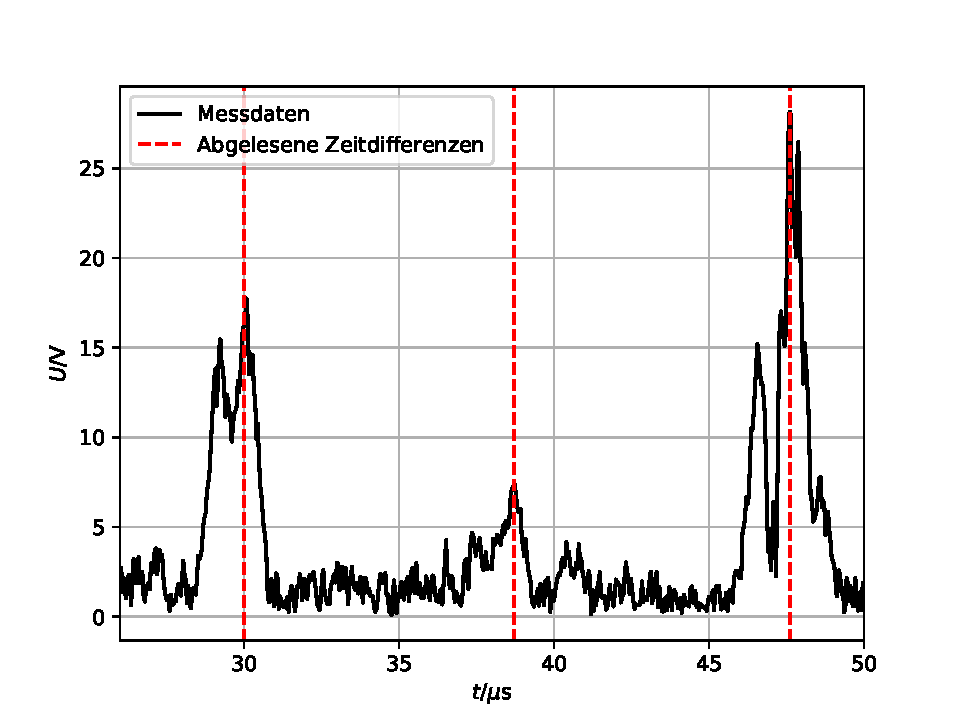
\includegraphics[width = 0.7\textwidth]{../Messdaten/plots/cepstrum.pdf}
  \caption{Graphische Darstellung des Cepstrums. Zeitliche Differenz $t$ und Amplitude $U$.}
  \label{fig: cepstrum}
\end{figure}

\begin{figure}[H]
  \centering
  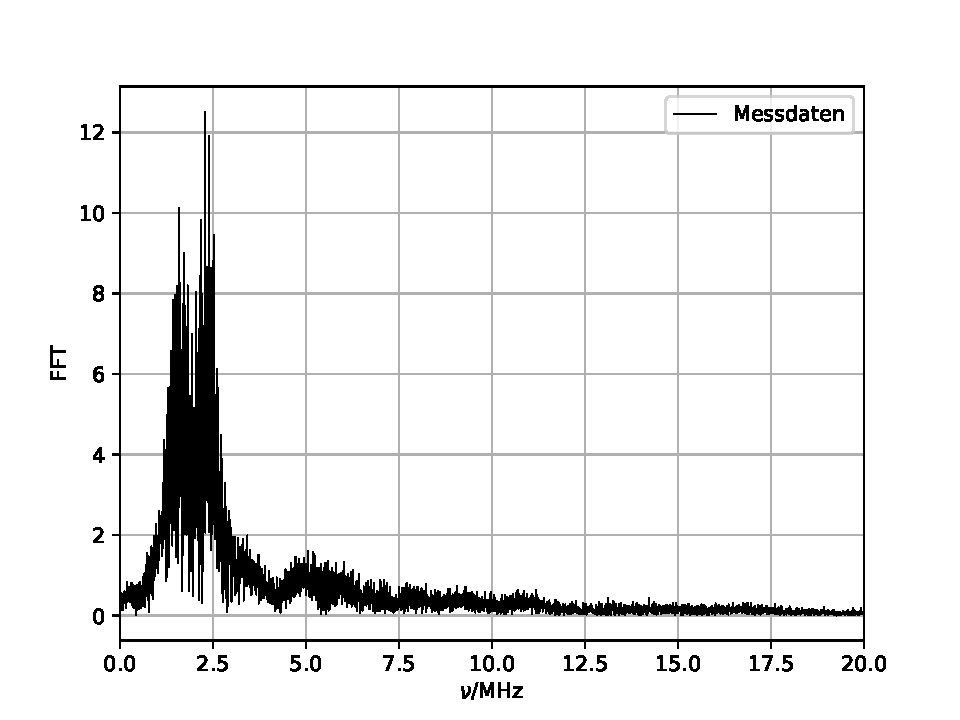
\includegraphics[width = 0.7\textwidth]{../Messdaten/plots/spectrum.pdf}
  \caption{Spektrum. Frequenz $\nu$ und FFT.}
  \label{fig: spektrum}
\end{figure}

\subsection{Längenmessung am Augenmodell}
Die aufgenommenen Daten zur Längenmessung am Augenmodell sind in Abbildung \ref{fig: auge} dargestellt. Die mit Hilfe
der Messsoftware bestimmten zeitlichen Koordinaten der erkennbaren Peaks sind in Tabelle \ref{tab: auge} aufgeführt, sowie in Abbildung
\ref{fig: auge} eingezeichnet. Hierbei werden die Peaks als Reflexionen an Hornhaut, Linse und Retina interpretiert. %Sollten nicht 5 Peaks erkennbar sein: Hornhaut, Iris, Linse eingang, Linse ausgang unf die Retina?
Mit Hilfe der aus der Anleitung \cite{anleitungus1} entnommenen Schallgeschwindigkeiten
\begin{align}
  \begin{aligned}
    c\ua{L} &= \SI{2500}{\meter\per\second}\\
    c\ua{GK}&= \SI{1410}{\meter\per\second}
  \end{aligned}
\end{align}
werden die räumlichen Abmessungen der Bestandteile berechnet. Hierbei entspricht $c\ua{L}$ der Schallgeschwindigkeit
in der Linse und $c\ua{GK}$ der in der Glaskörperflüssigkeit. Es ergeben sich
\begin{align}
  \begin{aligned}
a_1 &= \frac{t_2 - t_1}{2} c\ua{GK} &=&\,\, \SI[]{6.8}{\milli\meter} \\
a_2 &= \frac{t_3 - t_2}{2} c\ua{GK} &=&\,\, \SI[]{3.7}{\milli\meter}\\
a_3 &= \frac{t_4 - t_3}{2} c\ua{L}  &=&\,\, \SI[]{8.5}{\milli\meter}\\
a_4 &= \frac{t_5 - t_4}{2} c\ua{GK} &=&\,\,\SI[]{35.1}{\milli\meter}.
\end{aligned}
\end{align} .
Mit der Dicke der Hornhaut-Iris $a_1$, dem Abstand Iris-Linse $a_2$,
der Dicke der Linse $a_3$ und dem Abstand Linse-Retina $a_4$.
\begin{table}[H] 
\centering 
\caption{Daten zur Vermessung des Augenmodells. Zeitliche Abstände $t$ der Impulse zum Ursprung.} 
\label{tab: auge} 
\begin{tabular}{S S } 
\toprule  
{Puls} & {$t / \si{\micro\second}$}  \\ 
\midrule  
 1  & 1.1\\ 
2  & 10.8\\ 
3  & 16.0\\ 
4  & 22.8\\ 
5  & 72.6\\ 
\bottomrule 
\end{tabular} 
\end{table}
\begin{figure}[H]
  \centering
  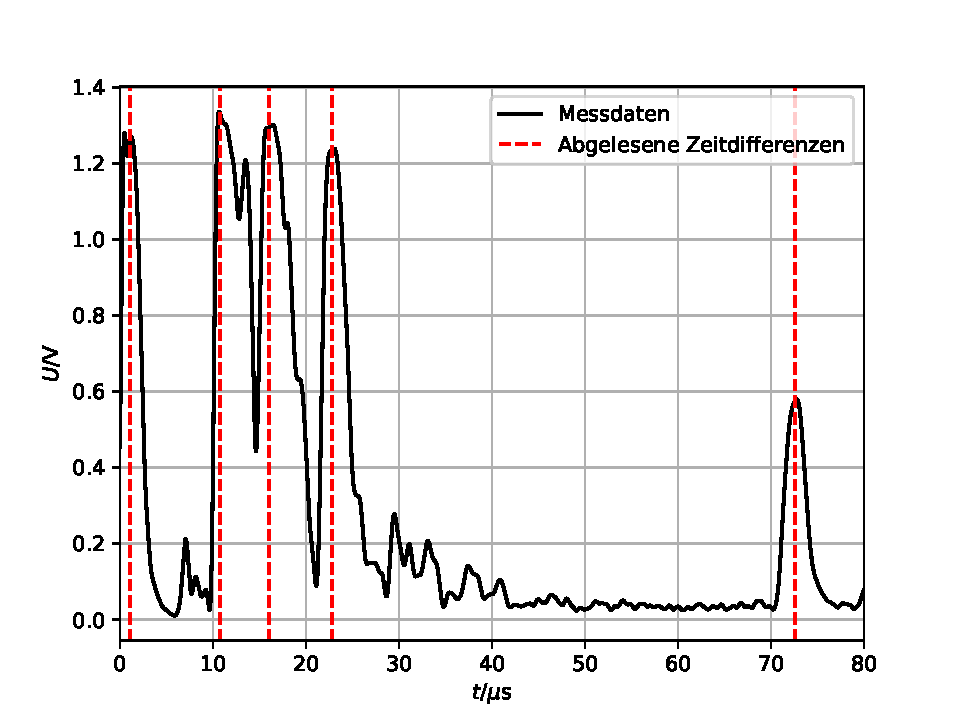
\includegraphics[width = 0.7\textwidth]{../Messdaten/plots/auge.pdf}
  \caption{Graphische Darstellung der aufgenommenen Messwerte zur Untersuchung des Augenmodells. Zeitlicher Abstand $t$ und Amplitude $U$.}
  \label{fig: auge}
\end{figure}
